% Created by tikzDevice version 0.7.0 on 2014-09-22 20:46:07
% !TEX encoding = UTF-8 Unicode
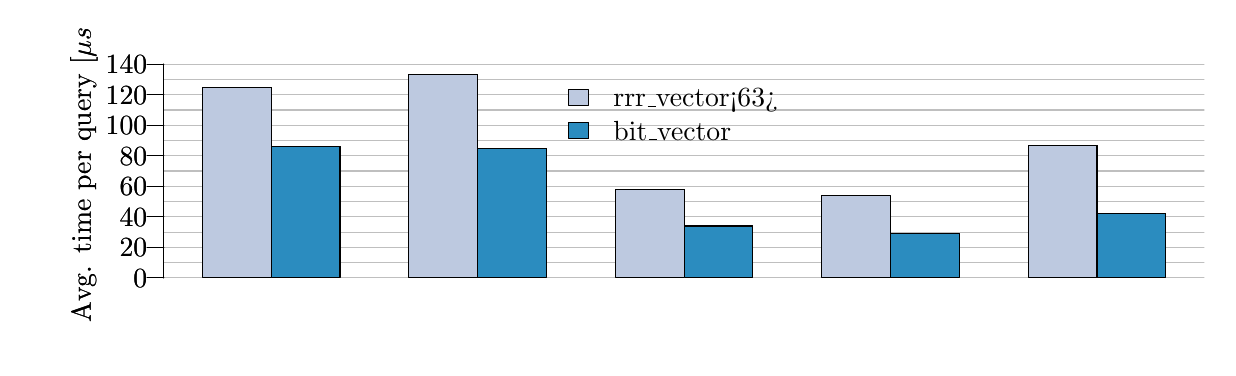
\begin{tikzpicture}[x=1pt,y=1pt]
\definecolor[named]{fillColor}{rgb}{1.00,1.00,1.00}
\path[use as bounding box,fill=fillColor,fill opacity=0.00] (0,0) rectangle (426.39,115.63);
\begin{scope}
\path[clip] (  0.00,  0.00) rectangle (426.39,115.63);
\definecolor[named]{drawColor}{rgb}{0.00,0.00,0.00}
\definecolor[named]{fillColor}{rgb}{0.74,0.79,0.88}

\path[draw=drawColor,line width= 0.4pt,line join=round,line cap=round,fill=fillColor] ( 63.13, 25.20) rectangle ( 87.99, 94.16);
\definecolor[named]{fillColor}{rgb}{0.17,0.55,0.75}

\path[draw=drawColor,line width= 0.4pt,line join=round,line cap=round,fill=fillColor] ( 87.99, 25.20) rectangle (112.86, 72.64);
\definecolor[named]{fillColor}{rgb}{0.74,0.79,0.88}

\path[draw=drawColor,line width= 0.4pt,line join=round,line cap=round,fill=fillColor] (137.73, 25.20) rectangle (162.59, 98.57);
\definecolor[named]{fillColor}{rgb}{0.17,0.55,0.75}

\path[draw=drawColor,line width= 0.4pt,line join=round,line cap=round,fill=fillColor] (162.59, 25.20) rectangle (187.46, 72.09);
\definecolor[named]{fillColor}{rgb}{0.74,0.79,0.88}

\path[draw=drawColor,line width= 0.4pt,line join=round,line cap=round,fill=fillColor] (212.33, 25.20) rectangle (237.20, 57.20);
\definecolor[named]{fillColor}{rgb}{0.17,0.55,0.75}

\path[draw=drawColor,line width= 0.4pt,line join=round,line cap=round,fill=fillColor] (237.20, 25.20) rectangle (262.06, 43.96);
\definecolor[named]{fillColor}{rgb}{0.74,0.79,0.88}

\path[draw=drawColor,line width= 0.4pt,line join=round,line cap=round,fill=fillColor] (286.93, 25.20) rectangle (311.80, 54.99);
\definecolor[named]{fillColor}{rgb}{0.17,0.55,0.75}

\path[draw=drawColor,line width= 0.4pt,line join=round,line cap=round,fill=fillColor] (311.80, 25.20) rectangle (336.67, 41.20);
\definecolor[named]{fillColor}{rgb}{0.74,0.79,0.88}

\path[draw=drawColor,line width= 0.4pt,line join=round,line cap=round,fill=fillColor] (361.53, 25.20) rectangle (386.40, 73.19);
\definecolor[named]{fillColor}{rgb}{0.17,0.55,0.75}

\path[draw=drawColor,line width= 0.4pt,line join=round,line cap=round,fill=fillColor] (386.40, 25.20) rectangle (411.27, 48.37);
\end{scope}
\begin{scope}
\path[clip] (  0.00,  0.00) rectangle (426.39,115.63);
\definecolor[named]{drawColor}{rgb}{0.00,0.00,0.00}

\node[text=drawColor,anchor=base,inner sep=0pt, outer sep=0pt, scale=  1.00] at ( 87.99,  9.60) {\ENWIKISML};

\node[text=drawColor,anchor=base,inner sep=0pt, outer sep=0pt, scale=  1.00] at (162.59,  9.60) {\ENWIKIBIG};

\node[text=drawColor,anchor=base,inner sep=0pt, outer sep=0pt, scale=  1.00] at (237.20,  9.60) {\ENWIKISMLINT};

\node[text=drawColor,anchor=base,inner sep=0pt, outer sep=0pt, scale=  1.00] at (311.80,  9.60) {\ENWIKIBIGINT};

\node[text=drawColor,anchor=base,inner sep=0pt, outer sep=0pt, scale=  1.00] at (386.40,  9.60) {\GOVII};
\end{scope}
\begin{scope}
\path[clip] (  0.00,  0.00) rectangle (426.39,115.63);
\definecolor[named]{drawColor}{rgb}{0.00,0.00,0.00}

\node[text=drawColor,rotate= 90.00,anchor=base,inner sep=0pt, outer sep=0pt, scale=  1.00] at ( 22.80, 63.82) {Avg. time per query [$\mu s$]};
\end{scope}
\begin{scope}
\path[clip] (  0.00,  0.00) rectangle (426.39,115.63);
\definecolor[named]{drawColor}{rgb}{0.00,0.00,0.00}

\path[draw=drawColor,line width= 0.4pt,line join=round,line cap=round] ( 49.20, 25.20) -- ( 49.20,102.43);

\path[draw=drawColor,line width= 0.4pt,line join=round,line cap=round] ( 49.20, 25.20) -- ( 43.20, 25.20);

\path[draw=drawColor,line width= 0.4pt,line join=round,line cap=round] ( 49.20, 36.23) -- ( 43.20, 36.23);

\path[draw=drawColor,line width= 0.4pt,line join=round,line cap=round] ( 49.20, 47.27) -- ( 43.20, 47.27);

\path[draw=drawColor,line width= 0.4pt,line join=round,line cap=round] ( 49.20, 58.30) -- ( 43.20, 58.30);

\path[draw=drawColor,line width= 0.4pt,line join=round,line cap=round] ( 49.20, 69.33) -- ( 43.20, 69.33);

\path[draw=drawColor,line width= 0.4pt,line join=round,line cap=round] ( 49.20, 80.37) -- ( 43.20, 80.37);

\path[draw=drawColor,line width= 0.4pt,line join=round,line cap=round] ( 49.20, 91.40) -- ( 43.20, 91.40);

\path[draw=drawColor,line width= 0.4pt,line join=round,line cap=round] ( 49.20,102.43) -- ( 43.20,102.43);

\node[text=drawColor,anchor=base east,inner sep=0pt, outer sep=0pt, scale=  1.00] at ( 43.20, 21.76) {0};

\node[text=drawColor,anchor=base east,inner sep=0pt, outer sep=0pt, scale=  1.00] at ( 43.20, 32.79) {20};

\node[text=drawColor,anchor=base east,inner sep=0pt, outer sep=0pt, scale=  1.00] at ( 43.20, 43.82) {40};

\node[text=drawColor,anchor=base east,inner sep=0pt, outer sep=0pt, scale=  1.00] at ( 43.20, 54.86) {60};

\node[text=drawColor,anchor=base east,inner sep=0pt, outer sep=0pt, scale=  1.00] at ( 43.20, 65.89) {80};

\node[text=drawColor,anchor=base east,inner sep=0pt, outer sep=0pt, scale=  1.00] at ( 43.20, 76.92) {100};

\node[text=drawColor,anchor=base east,inner sep=0pt, outer sep=0pt, scale=  1.00] at ( 43.20, 87.96) {120};

\node[text=drawColor,anchor=base east,inner sep=0pt, outer sep=0pt, scale=  1.00] at ( 43.20, 98.99) {140};
\end{scope}
\begin{scope}
\path[clip] ( 49.20, 25.20) rectangle (425.19,102.43);
\definecolor[named]{drawColor}{rgb}{0.75,0.75,0.75}

\path[draw=drawColor,line width= 0.4pt,line join=round,line cap=round] ( 49.20, 25.20) -- (425.19, 25.20);

\path[draw=drawColor,line width= 0.4pt,line join=round,line cap=round] ( 49.20, 30.72) -- (425.19, 30.72);

\path[draw=drawColor,line width= 0.4pt,line join=round,line cap=round] ( 49.20, 36.23) -- (425.19, 36.23);

\path[draw=drawColor,line width= 0.4pt,line join=round,line cap=round] ( 49.20, 41.75) -- (425.19, 41.75);

\path[draw=drawColor,line width= 0.4pt,line join=round,line cap=round] ( 49.20, 47.27) -- (425.19, 47.27);

\path[draw=drawColor,line width= 0.4pt,line join=round,line cap=round] ( 49.20, 52.78) -- (425.19, 52.78);

\path[draw=drawColor,line width= 0.4pt,line join=round,line cap=round] ( 49.20, 58.30) -- (425.19, 58.30);

\path[draw=drawColor,line width= 0.4pt,line join=round,line cap=round] ( 49.20, 63.82) -- (425.19, 63.82);

\path[draw=drawColor,line width= 0.4pt,line join=round,line cap=round] ( 49.20, 69.33) -- (425.19, 69.33);

\path[draw=drawColor,line width= 0.4pt,line join=round,line cap=round] ( 49.20, 74.85) -- (425.19, 74.85);

\path[draw=drawColor,line width= 0.4pt,line join=round,line cap=round] ( 49.20, 80.37) -- (425.19, 80.37);

\path[draw=drawColor,line width= 0.4pt,line join=round,line cap=round] ( 49.20, 85.88) -- (425.19, 85.88);

\path[draw=drawColor,line width= 0.4pt,line join=round,line cap=round] ( 49.20, 91.40) -- (425.19, 91.40);

\path[draw=drawColor,line width= 0.4pt,line join=round,line cap=round] ( 49.20, 96.92) -- (425.19, 96.92);

\path[draw=drawColor,line width= 0.4pt,line join=round,line cap=round] ( 49.20,102.43) -- (425.19,102.43);
\end{scope}
\begin{scope}
\path[clip] (  0.00,  0.00) rectangle (426.39,115.63);
\definecolor[named]{drawColor}{rgb}{0.00,0.00,0.00}
\definecolor[named]{fillColor}{rgb}{0.74,0.79,0.88}

\path[draw=drawColor,line width= 0.4pt,line join=round,line cap=round,fill=fillColor] ( 63.13, 25.20) rectangle ( 87.99, 94.16);
\definecolor[named]{fillColor}{rgb}{0.17,0.55,0.75}

\path[draw=drawColor,line width= 0.4pt,line join=round,line cap=round,fill=fillColor] ( 87.99, 25.20) rectangle (112.86, 72.64);
\definecolor[named]{fillColor}{rgb}{0.74,0.79,0.88}

\path[draw=drawColor,line width= 0.4pt,line join=round,line cap=round,fill=fillColor] (137.73, 25.20) rectangle (162.59, 98.57);
\definecolor[named]{fillColor}{rgb}{0.17,0.55,0.75}

\path[draw=drawColor,line width= 0.4pt,line join=round,line cap=round,fill=fillColor] (162.59, 25.20) rectangle (187.46, 72.09);
\definecolor[named]{fillColor}{rgb}{0.74,0.79,0.88}

\path[draw=drawColor,line width= 0.4pt,line join=round,line cap=round,fill=fillColor] (212.33, 25.20) rectangle (237.20, 57.20);
\definecolor[named]{fillColor}{rgb}{0.17,0.55,0.75}

\path[draw=drawColor,line width= 0.4pt,line join=round,line cap=round,fill=fillColor] (237.20, 25.20) rectangle (262.06, 43.96);
\definecolor[named]{fillColor}{rgb}{0.74,0.79,0.88}

\path[draw=drawColor,line width= 0.4pt,line join=round,line cap=round,fill=fillColor] (286.93, 25.20) rectangle (311.80, 54.99);
\definecolor[named]{fillColor}{rgb}{0.17,0.55,0.75}

\path[draw=drawColor,line width= 0.4pt,line join=round,line cap=round,fill=fillColor] (311.80, 25.20) rectangle (336.67, 41.20);
\definecolor[named]{fillColor}{rgb}{0.74,0.79,0.88}

\path[draw=drawColor,line width= 0.4pt,line join=round,line cap=round,fill=fillColor] (361.53, 25.20) rectangle (386.40, 73.19);
\definecolor[named]{fillColor}{rgb}{0.17,0.55,0.75}

\path[draw=drawColor,line width= 0.4pt,line join=round,line cap=round,fill=fillColor] (386.40, 25.20) rectangle (411.27, 48.37);
\end{scope}
\begin{scope}
\path[clip] (  0.00,  0.00) rectangle (426.39,115.63);
\definecolor[named]{drawColor}{rgb}{0.00,0.00,0.00}

\node[text=drawColor,anchor=base,inner sep=0pt, outer sep=0pt, scale=  1.00] at ( 87.99,  9.60) {\ENWIKISML};

\node[text=drawColor,anchor=base,inner sep=0pt, outer sep=0pt, scale=  1.00] at (162.59,  9.60) {\ENWIKIBIG};

\node[text=drawColor,anchor=base,inner sep=0pt, outer sep=0pt, scale=  1.00] at (237.20,  9.60) {\ENWIKISMLINT};

\node[text=drawColor,anchor=base,inner sep=0pt, outer sep=0pt, scale=  1.00] at (311.80,  9.60) {\ENWIKIBIGINT};

\node[text=drawColor,anchor=base,inner sep=0pt, outer sep=0pt, scale=  1.00] at (386.40,  9.60) {\GOVII};
\end{scope}
\begin{scope}
\path[clip] (  0.00,  0.00) rectangle (426.39,115.63);
\definecolor[named]{drawColor}{rgb}{0.00,0.00,0.00}

\node[text=drawColor,rotate= 90.00,anchor=base,inner sep=0pt, outer sep=0pt, scale=  1.00] at ( 22.80, 63.82) {Avg. time per query [$\mu s$]};
\end{scope}
\begin{scope}
\path[clip] (  0.00,  0.00) rectangle (426.39,115.63);
\definecolor[named]{drawColor}{rgb}{0.00,0.00,0.00}

\path[draw=drawColor,line width= 0.4pt,line join=round,line cap=round] ( 49.20, 25.20) -- ( 49.20,102.43);

\path[draw=drawColor,line width= 0.4pt,line join=round,line cap=round] ( 49.20, 25.20) -- ( 43.20, 25.20);

\path[draw=drawColor,line width= 0.4pt,line join=round,line cap=round] ( 49.20, 36.23) -- ( 43.20, 36.23);

\path[draw=drawColor,line width= 0.4pt,line join=round,line cap=round] ( 49.20, 47.27) -- ( 43.20, 47.27);

\path[draw=drawColor,line width= 0.4pt,line join=round,line cap=round] ( 49.20, 58.30) -- ( 43.20, 58.30);

\path[draw=drawColor,line width= 0.4pt,line join=round,line cap=round] ( 49.20, 69.33) -- ( 43.20, 69.33);

\path[draw=drawColor,line width= 0.4pt,line join=round,line cap=round] ( 49.20, 80.37) -- ( 43.20, 80.37);

\path[draw=drawColor,line width= 0.4pt,line join=round,line cap=round] ( 49.20, 91.40) -- ( 43.20, 91.40);

\path[draw=drawColor,line width= 0.4pt,line join=round,line cap=round] ( 49.20,102.43) -- ( 43.20,102.43);

\node[text=drawColor,anchor=base east,inner sep=0pt, outer sep=0pt, scale=  1.00] at ( 43.20, 21.76) {0};

\node[text=drawColor,anchor=base east,inner sep=0pt, outer sep=0pt, scale=  1.00] at ( 43.20, 32.79) {20};

\node[text=drawColor,anchor=base east,inner sep=0pt, outer sep=0pt, scale=  1.00] at ( 43.20, 43.82) {40};

\node[text=drawColor,anchor=base east,inner sep=0pt, outer sep=0pt, scale=  1.00] at ( 43.20, 54.86) {60};

\node[text=drawColor,anchor=base east,inner sep=0pt, outer sep=0pt, scale=  1.00] at ( 43.20, 65.89) {80};

\node[text=drawColor,anchor=base east,inner sep=0pt, outer sep=0pt, scale=  1.00] at ( 43.20, 76.92) {100};

\node[text=drawColor,anchor=base east,inner sep=0pt, outer sep=0pt, scale=  1.00] at ( 43.20, 87.96) {120};

\node[text=drawColor,anchor=base east,inner sep=0pt, outer sep=0pt, scale=  1.00] at ( 43.20, 98.99) {140};
\end{scope}
\begin{scope}
\path[clip] ( 49.20, 25.20) rectangle (425.19,102.43);
\definecolor[named]{drawColor}{rgb}{0.00,0.00,0.00}
\definecolor[named]{fillColor}{rgb}{0.74,0.79,0.88}

\path[draw=drawColor,line width= 0.4pt,line join=round,line cap=round,fill=fillColor] (195.47, 93.43) rectangle (202.67, 87.43);
\definecolor[named]{fillColor}{rgb}{0.17,0.55,0.75}

\path[draw=drawColor,line width= 0.4pt,line join=round,line cap=round,fill=fillColor] (195.47, 81.43) rectangle (202.67, 75.43);

\node[text=drawColor,anchor=base west,inner sep=0pt, outer sep=0pt, scale=  1.00] at (211.67, 86.99) {rrr\_vector<63>};

\node[text=drawColor,anchor=base west,inner sep=0pt, outer sep=0pt, scale=  1.00] at (211.67, 74.99) {bit\_vector};
\end{scope}
\end{tikzpicture}
